% course:       CV
% teacher:      DongHui Wang
% author:       zju_cs / Yi Zhang / 21721190
% mail:         yizhangzc@gmail.com
% data:         2018/5
% environment:  ubuntu 16.04 / texlive-full / texlive-xetex      
% compiler:     xelatex / bibtex

\documentclass[a4paper]{article}

\usepackage{ctex}           % support chinese
\usepackage{geometry}       % setting margin
\usepackage{setspace}       % setting space
\usepackage{graphicx}       % support insert iamge
\usepackage{subcaption}


\title{CNN for AffNIST classification}
\date{2018-05}
\author{张毅\hspace{1em}21721190}

\geometry{left=3cm,right=3cm,top=2.5cm,bottom=2.5cm}

\begin{document}

    \pagenumbering{gobble}
    
    \begin{center}
        \doublespacing
        
        \Large \textbf{CNN for AffNIST classification}

        \normalsize 姓名:张毅 \qquad 学号:21721190 \qquad 日期:2018-5
    \end{center}

    \section{问题描述}

    在AffNIST数据集上训练模型进行分类任务,识别0-9十个数字。

    数据集: AffNIST(https://www.cs.toronto.edu/~tijmen/affNIST/),训练数据与测试数据默认已经划分好,试验中采用默认的划分方式。

    \section{方法及原理}

    实验中采用了CNN(包括4个卷基层,1个全连接层与一个softmax层)进行分类,模型结构见tensorflow计算图,代码已经上传到github仓库(yizhangzc/course),本次实验与第一次实验代码均放置在classification文件夹下,运行方式及运行环境见README.md。

    \section{实验结果}

    本次实验在全部数据集上进行,结果如下:

        \begin{center}
            DNN:\qquad 准确率:98.8\% \qquad f1值:98.8\%
        \end{center}

        \begin{figure}[htbp]
            \centering
            \begin{subfigure}[b]{0.48\textwidth}
                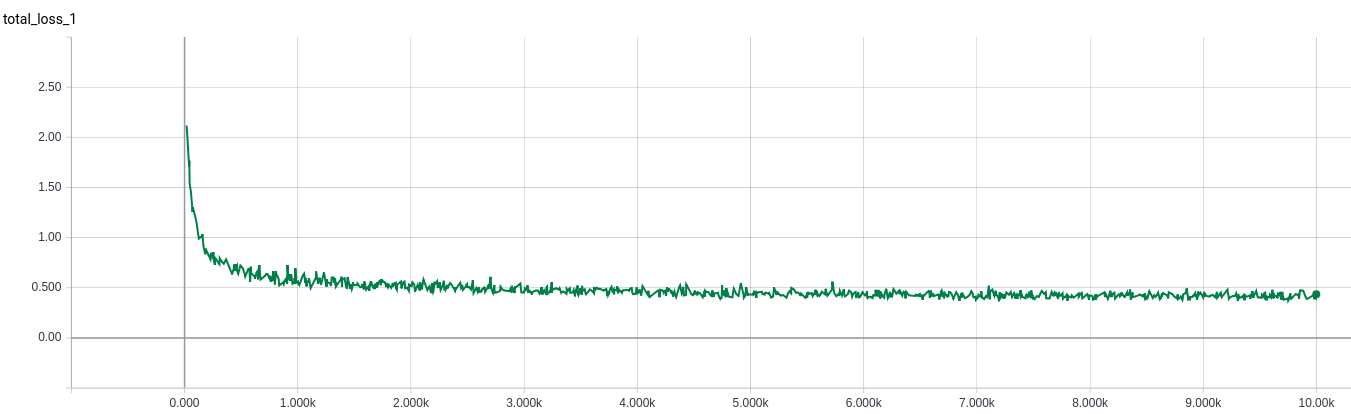
\includegraphics[width=\textwidth]{./images/total_loss_dnn.png}
                \caption{loss下降过程}
            \end{subfigure}
            \begin{subfigure}[b]{0.48\textwidth}
                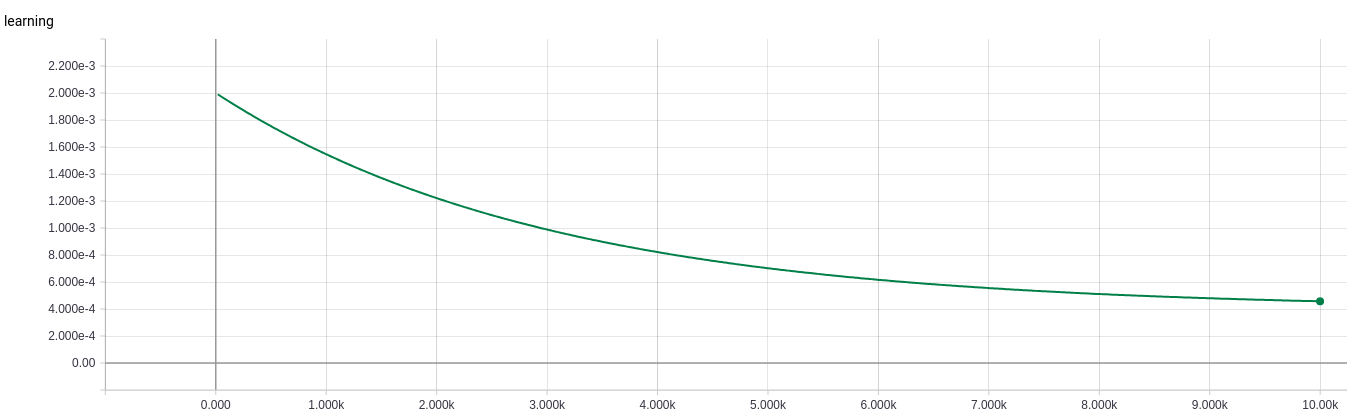
\includegraphics[width=\textwidth]{./images/learning_rate_dnn.png}
                \caption{学习速率下降过程}
            \end{subfigure}

            \begin{subfigure}[b]{0.6\textwidth}
                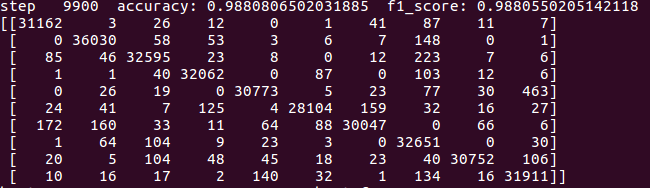
\includegraphics[width=\textwidth]{./images/confusion_matrix_dnn.png}
                \caption{DNN混淆矩阵}
            \end{subfigure}
            
            \label{fig:confusion_matrix}
        \end{figure}

        当与第一次实验使用相同数据量(每个.mat文件中均取1000个样本),CNN模型的识别准确率可以达到97.1\%,大大超过KNN的68.8\%和SVM的82.2\%。

    \section{总结}

    (1)batch normalization有效的加快了训练过程,提高了模型的性能。(2)模型学习速率可变能够使模型训练过程更好,实验中,采用了按指数规律下降的学习速率。(3)使用tensorboard能监控模型训练过程,对debug有帮助。(4)模型训练采用了传统的交叉熵损失结合L2\_norm防止过拟合,采用Adam优化器。(5)为防止过拟合还引入了dropout。(6)模型结果受参数初始化以及batch大小等影响,每次不完全相同,但大致相近。实验中batch大小取100。

    \section{计算图}

    \begin{figure}[htbp]
        \centering
        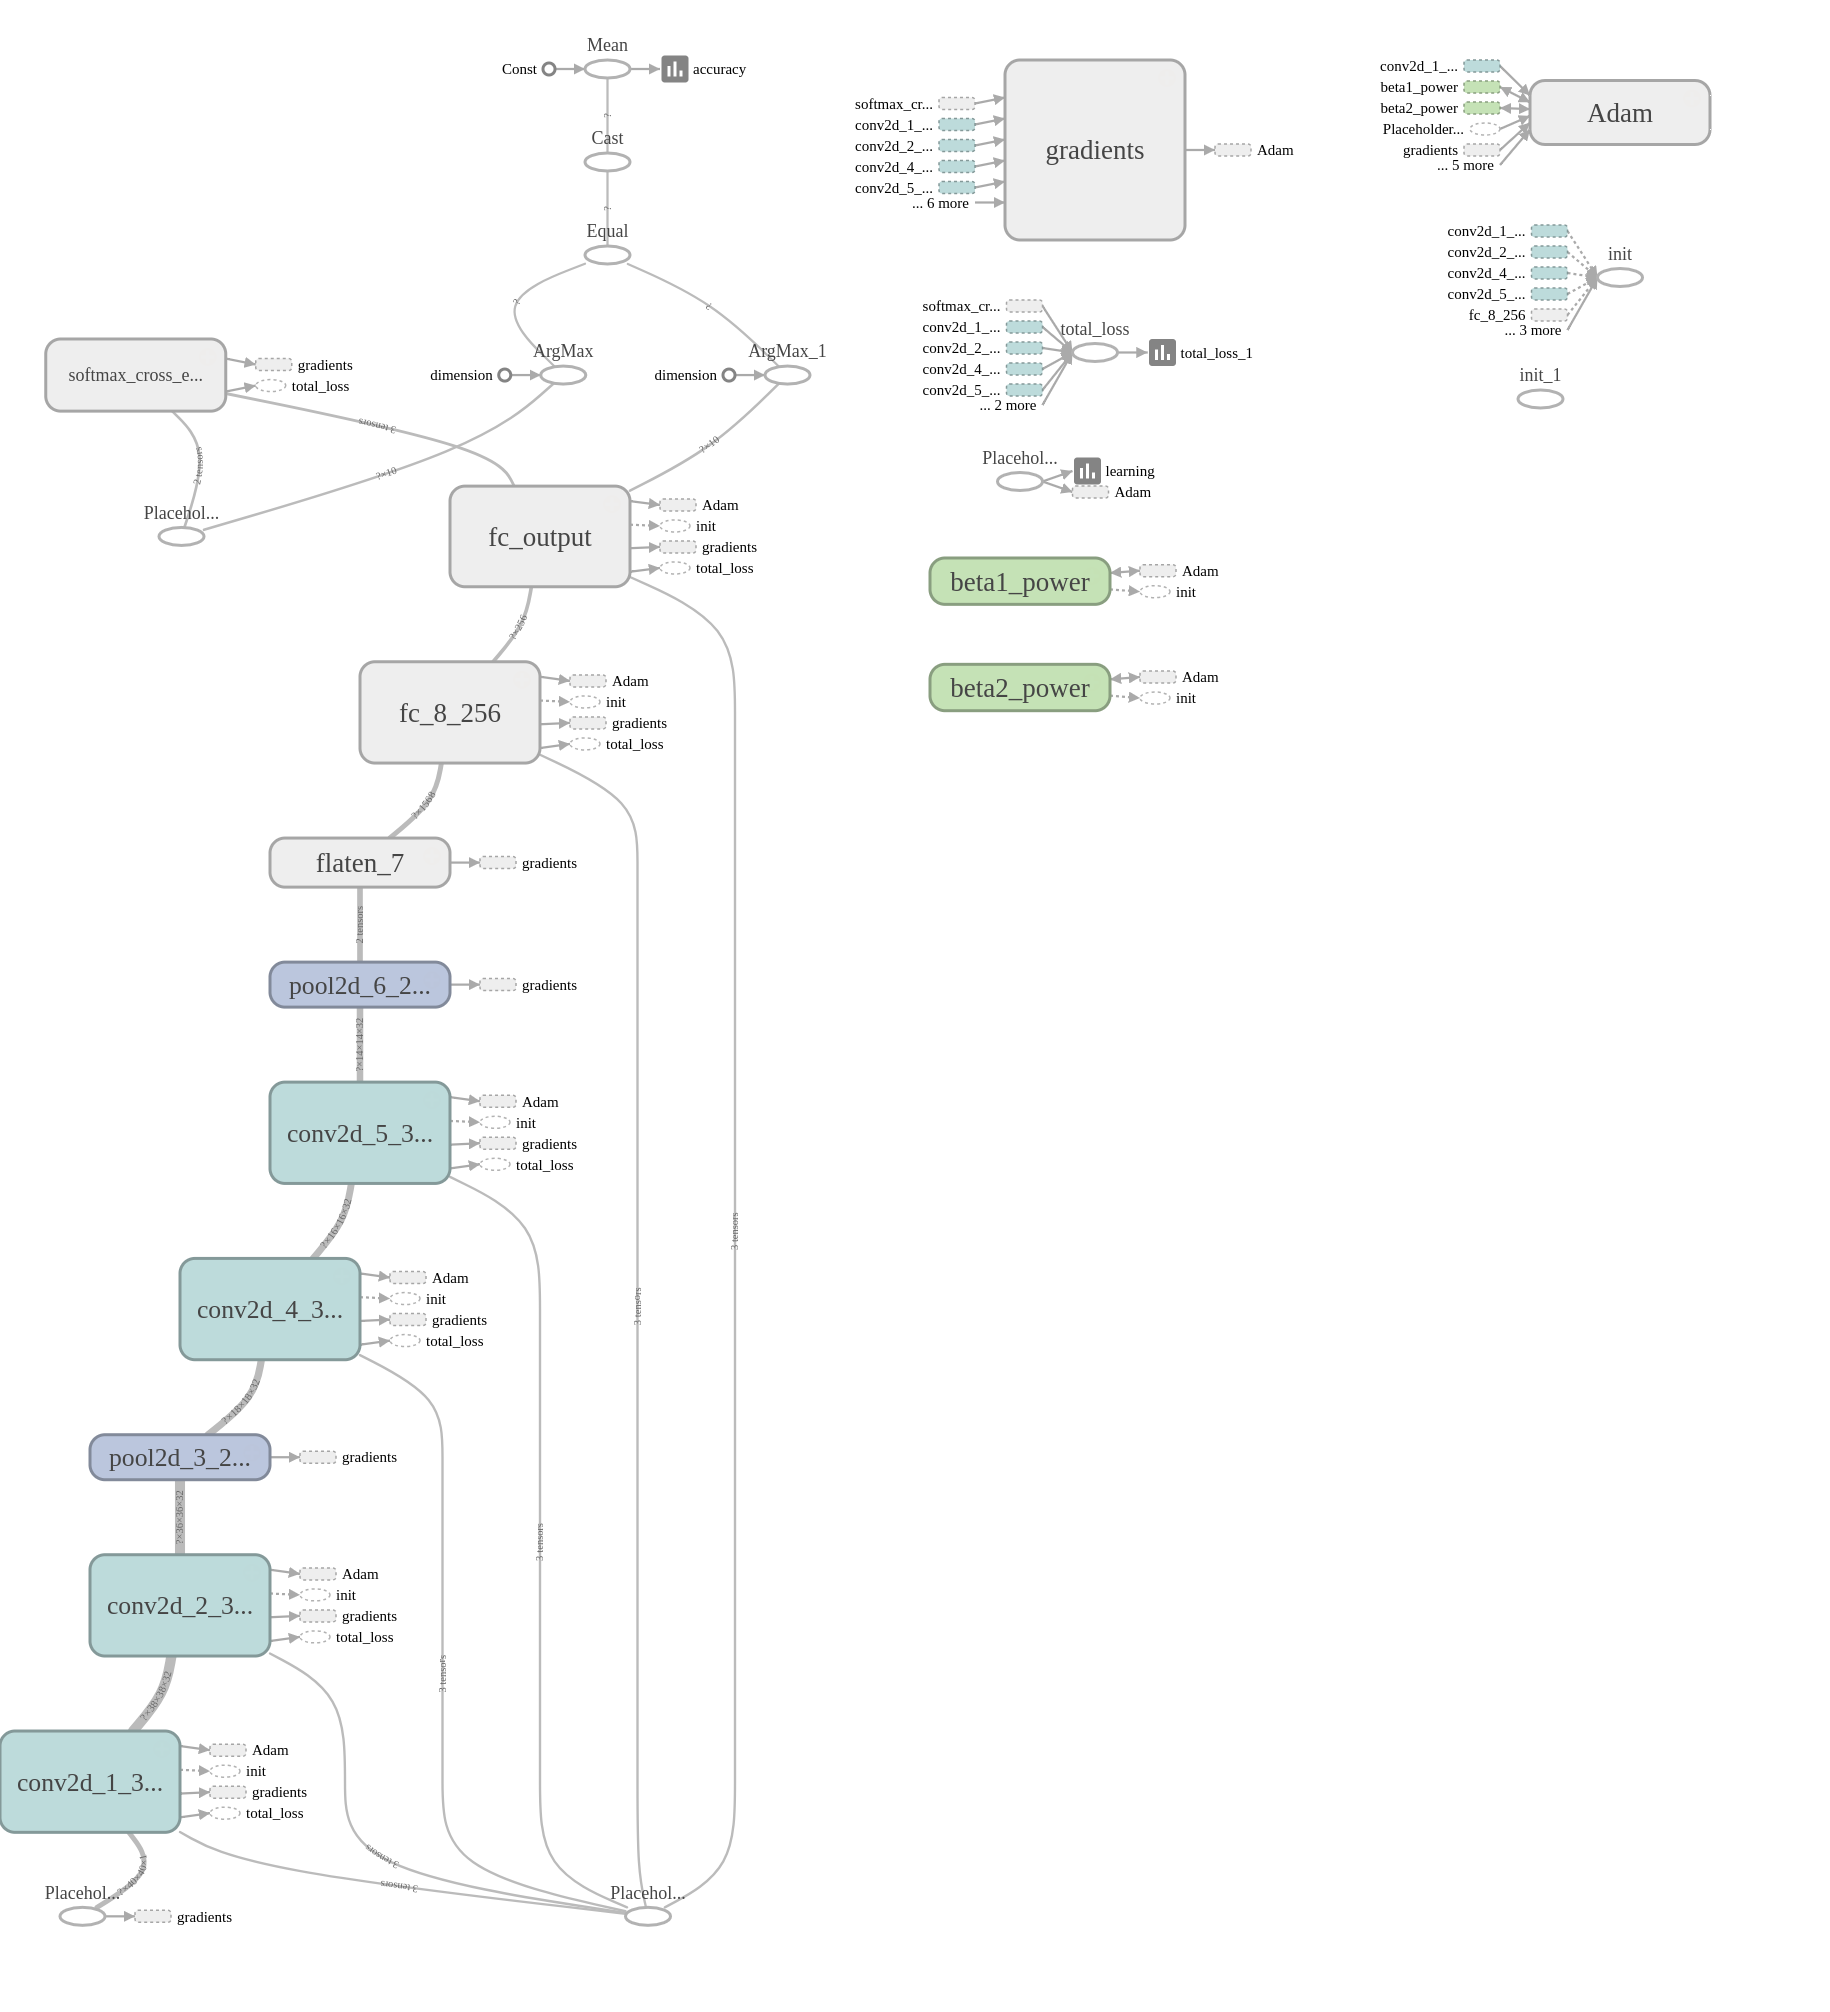
\includegraphics[width=\linewidth]{./images/graph_dnn.png}
        \caption{DNN计算图(tensorflow自动生成)}
        \label{fig:confusion_matrix}
    \end{figure}
    
\end{document}